% Prof. Dr. Ausberto S. Castro Vera
% UENF - CCT - LCMAT - Curso de Ci\^{e}ncia da Computa\c{c}\~{a}o
% Campos, RJ,  2023 
% Disciplina: An\'{a}lise e Projeto de Sistemas
% Aluno:

\chapterimage{projeto.png} % Table of contents heading image
\chapter{Projeto do Sistema}

Exploraremos a estratégia definida para o desenvolvimento do sistema de gerenciamento de concessionárias de motos. Este projeto é uma parte fundamental na busca por soluções eficazes que aprimorem a administração das concessionárias e a experiência dos clientes. Discutiremos os objetivos do projeto, a metodologia de desenvolvimento, o cronograma, o orçamento e a equipe de projeto. Cada elemento da estratégia é crucial para garantir o sucesso da empreitada e a entrega de um sistema que atenda aos requisitos estabelecidos. Vamos adentrar nas detalhes que direcionarão a realização deste projeto.


\section{Estratégia do Projeto}

O desenvolvimento do sistema de gerenciamento para concessionárias de motos é um projeto crucial que visa fornecer uma solução eficaz e eficiente para melhorar a gestão das concessionárias e aprimorar a experiência dos clientes. A estratégia do projeto é fundamental para garantir o sucesso e a conclusão dentro do escopo, prazo e orçamento definidos.

\subsection{Objetivos do Projeto}

Os principais objetivos do projeto são:

\begin{itemize}
	\item Desenvolver um Sistema Eficiente: O sistema deve ser eficiente e fácil de usar, permitindo que os funcionários da concessionária realizem tarefas de gerenciamento, como cadastro de clientes, registro de vendas e geração de relatórios, de forma simplificada e eficaz.
	
	\item Melhorar a Experiência do Cliente: O sistema deve melhorar a experiência dos clientes, acelerando o processo de compra de motos, fornecendo informações detalhadas sobre os produtos e facilitando o atendimento personalizado.
	
	\item Integração com o Banco de Dados: Garantir que o sistema esteja completamente integrado com o banco de dados que armazena informações sobre clientes, motos e vendas. Isso permite que os dados sejam atualizados em tempo real e fornece uma base sólida para relatórios detalhados.
	
	\item Aprimorar a Gestão de Estoque: O sistema deve fornecer funcionalidades de gerenciamento de estoque para garantir que a concessionária mantenha um controle preciso do inventário de motos disponíveis.
	
	\item Facilitar a Análise de Desempenho: O sistema deve permitir a geração de relatórios detalhados de vendas, fornecendo informações valiosas para análise de desempenho e tomada de decisões.
\end{itemize}

\subsection{Metodologia de Desenvolvimento}

Para a execução deste projeto, adotaremos uma abordagem de desenvolvimento ágil, uma metodologia amplamente reconhecida pela sua eficiência e flexibilidade. Esta abordagem implica na divisão do projeto em iterações, cada uma delas focada em uma funcionalidade específica. Isso permite que as equipes de desenvolvimento trabalhem em colaboração, garantindo que o sistema evolua gradualmente de acordo com as necessidades do usuário.

O processo ágil é caracterizado pela revisão contínua e pela capacidade de fazer ajustes à medida que o projeto avança. Isso significa que estamos preparados para adaptar o sistema às mudanças que possam surgir durante o desenvolvimento, garantindo que ele permaneça alinhado com os requisitos e objetivos do projeto. Essa flexibilidade é fundamental para o sucesso do projeto e a satisfação do cliente, uma vez que permite a incorporação de feedback em tempo real e a entrega de um sistema que realmente atende às necessidades da concessionária e dos clientes.

\subsection{Cronograma}

O projeto seguirá o seguinte cronograma:

O cronograma apresenta um roteiro claro para o desenvolvimento do Sistema de Gerenciamento de Concessionárias de Motos, detalhando as atividades ao longo das 37 semanas do projeto.

\begin{figure}[h]
	\centering
	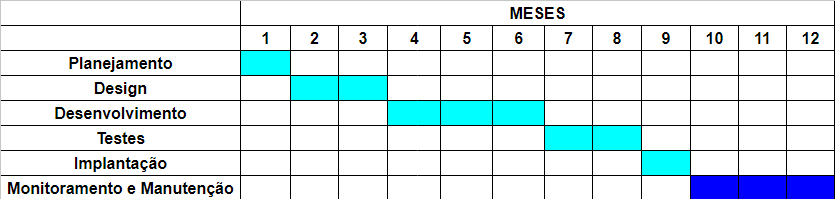
\includegraphics[width=\textwidth]{cronograma.png}
	\caption{Cronograma do Projeto}
	\label{fig:cronograma}
\end{figure}

Planejamento de atividades ao longo das próximas semanas, fornecendo uma visão abrangente do cronograma do projeto.
\begin{enumerate}
	\item Fase de Planejamento (Duração: 4 semanas)
	\begin{itemize}
		\item Identificação de Requisitos e Análise de Necessidades (2 semanas)
		\item Definição de Escopo e Objetivos (1 semana)
		\item Elaboração do Plano de Projeto (1 semana)
	\end{itemize}
	
	\item Fase de Design (Duração: 6 semanas)
	\begin{itemize}
		\item Design da Interface do Usuário (2 semanas)
		\item Arquitetura de Software e Banco de Dados (2 semanas)
		\item Especificações Técnicas (2 semanas)
	\end{itemize}
	
	\item Fase de Desenvolvimento (Duração: 12 semanas)
	\begin{itemize}
		\item Desenvolvimento do Software (8 semanas)
		\item Testes Unitários (2 semanas)
		\item Integração de Módulos (2 semanas)
	\end{itemize}
	
	\item Fase de Testes (Duração: 8 semanas)
	\begin{itemize}
		\item Testes de Aceitação do Usuário (4 semanas)
		\item Testes de Desempenho (2 semanas)
		\item Correções e Ajustes (2 semanas)
	\end{itemize}
	
	\item Fase de Implantação (Duração: 4 semanas)
	\begin{itemize}
		\item Treinamento de Usuários (2 semanas)
		\item Preparação para Lançamento (1 semana)
		\item Implantação do Sistema (1 semana)
	\end{itemize}
	
	\item Fase de Monitoramento e Manutenção (Duração: Contínua após a implantação)
	\begin{itemize}
		\item Suporte Técnico (em curso)
		\item Atualizações de Software (em curso)
		\item Monitoramento de Desempenho (em curso)
	\end{itemize}
	
\end{enumerate}

\subsection{Orçamento}

O orçamento para este projeto inclui custos de desenvolvimento de software, custos de treinamento e despesas operacionais. O orçamento total estimado é de R\$ 200.000.

\subsection{Equipe do Projeto}

A equipe do projeto é composta por desenvolvedores de software, analistas de negócios, gerentes de projeto e especialistas em banco de dados. Cada membro da equipe desempenha um papel vital na concepção, desenvolvimento e implementação do sistema.

A estratégia do projeto estabelecida visa cumprir os objetivos e fornecer um sistema de alta qualidade que atenda às necessidades das concessionárias e clientes. A próxima seção abordará os requisitos detalhados do sistema.


\section{Refinamento dos Diagramas DFD e E-R}


\section{Arquitetura do Sistema - Estilos}

    Utilize o PowerPoint para fazer a arquitetura(s) do sistema!!!

    \subsection{Arquitetura do Sistema}



    \subsection{Arquitetura do Hardware}


    \subsection{Arquitetura de Software}


\section{Projeto de Interface}


